Implementace pro více procesů byla implementována přes knihovnu \textit{OpenMPI}.
Implementace byla typu mater/slave.
Master zajišťoval běh programu, příjimal a rozesílal úlohy od/k slave procesům a spravoval globálně maximální dosaženou hodnotu vah.
Slave procesy naopak přijímaly požadavky k výpočtu od Master procesu.
Každý Slave proces prováděl výpočet pomocí \textit{Data paralelismu} blíže popsaným dříve.
Master proces nejprve rozeslal všem Slave procesům úlohy a poté ve \verb|while| smyčce čekal na odpověď některého z nich. Jakmile odpověď přišla, Master si uložil případné nové dosavadní maximum
a témuž procesu ihned vrátil další úlohu k vypočtení s již aktualizovaným dosavadním maximem.
To Master proces opakoval dokud ještě byla práce.
Po vypočtení všech úloh bylo rozesláno z Master procesu všem Slave procesům požadavek, aby se ukončili.

Při výpočtu je třeba nastavit dvě konfigurace
a těmi jsou počet disjunktních stavů získaných z BFS na úrovni Master procesu a na úrovni Slave procesů.
Experimentálně byly nastaveny tyto hodnoty na 50 resp. 200.

Pro vylepšení MPI úlohy může značně pomoci rozesílání nově nalezeného maxima rovnou ostatním Slave procesům i Master procesu. Druhým výrazným zlepšením může být zaměstnání zbývajícich jader na Master procesu.

Výsledky měření jsou zachyceny v následující tabulce. 
V porovnání oproti sekvenčnímu řešení jsou řešení až desetinásobně rychlejší.
Z grafu lze však vyčíst, že ke zrychlení přijde relativně rychle
a později už je zrychlení zanedbatelné.

\FloatBarrier
\begin{table}[]
    \begin{tabular}{l|rrr}
                    instance &   čas (s) &  počet jader &  počet procesů \\
    \hline
    graf\_15\_8.txt & 30.655 &           2 &         4 \\
    graf\_21\_6.txt & 58.113 &           2 &         4 \\
    graf\_18\_7.txt & 74.483 &           2 &         4 \\
    graf\_15\_8.txt & 17.470 &           4 &         4 \\
    graf\_21\_6.txt & 25.424 &           4 &         4 \\
    graf\_18\_7.txt & 41.837 &           4 &         4 \\
    graf\_15\_8.txt & 11.649 &           8 &         4 \\
    graf\_21\_6.txt & 17.472 &           8 &         4 \\
    graf\_18\_7.txt & 28.435 &           8 &         4 \\
    graf\_15\_8.txt & 10.057 &          16 &         4 \\
    graf\_21\_6.txt & 14.757 &          16 &         4 \\
    graf\_18\_7.txt & 23.623 &          16 &         4 \\
    graf\_15\_8.txt &  9.818 &          20 &         4 \\
    graf\_21\_6.txt & 15.157 &          20 &         4 \\
    graf\_18\_7.txt & 23.019 &          20 &         4 \\
    \end{tabular}
\end{table}
\FloatBarrier


\begin{figure}[!htbp]
\centerline{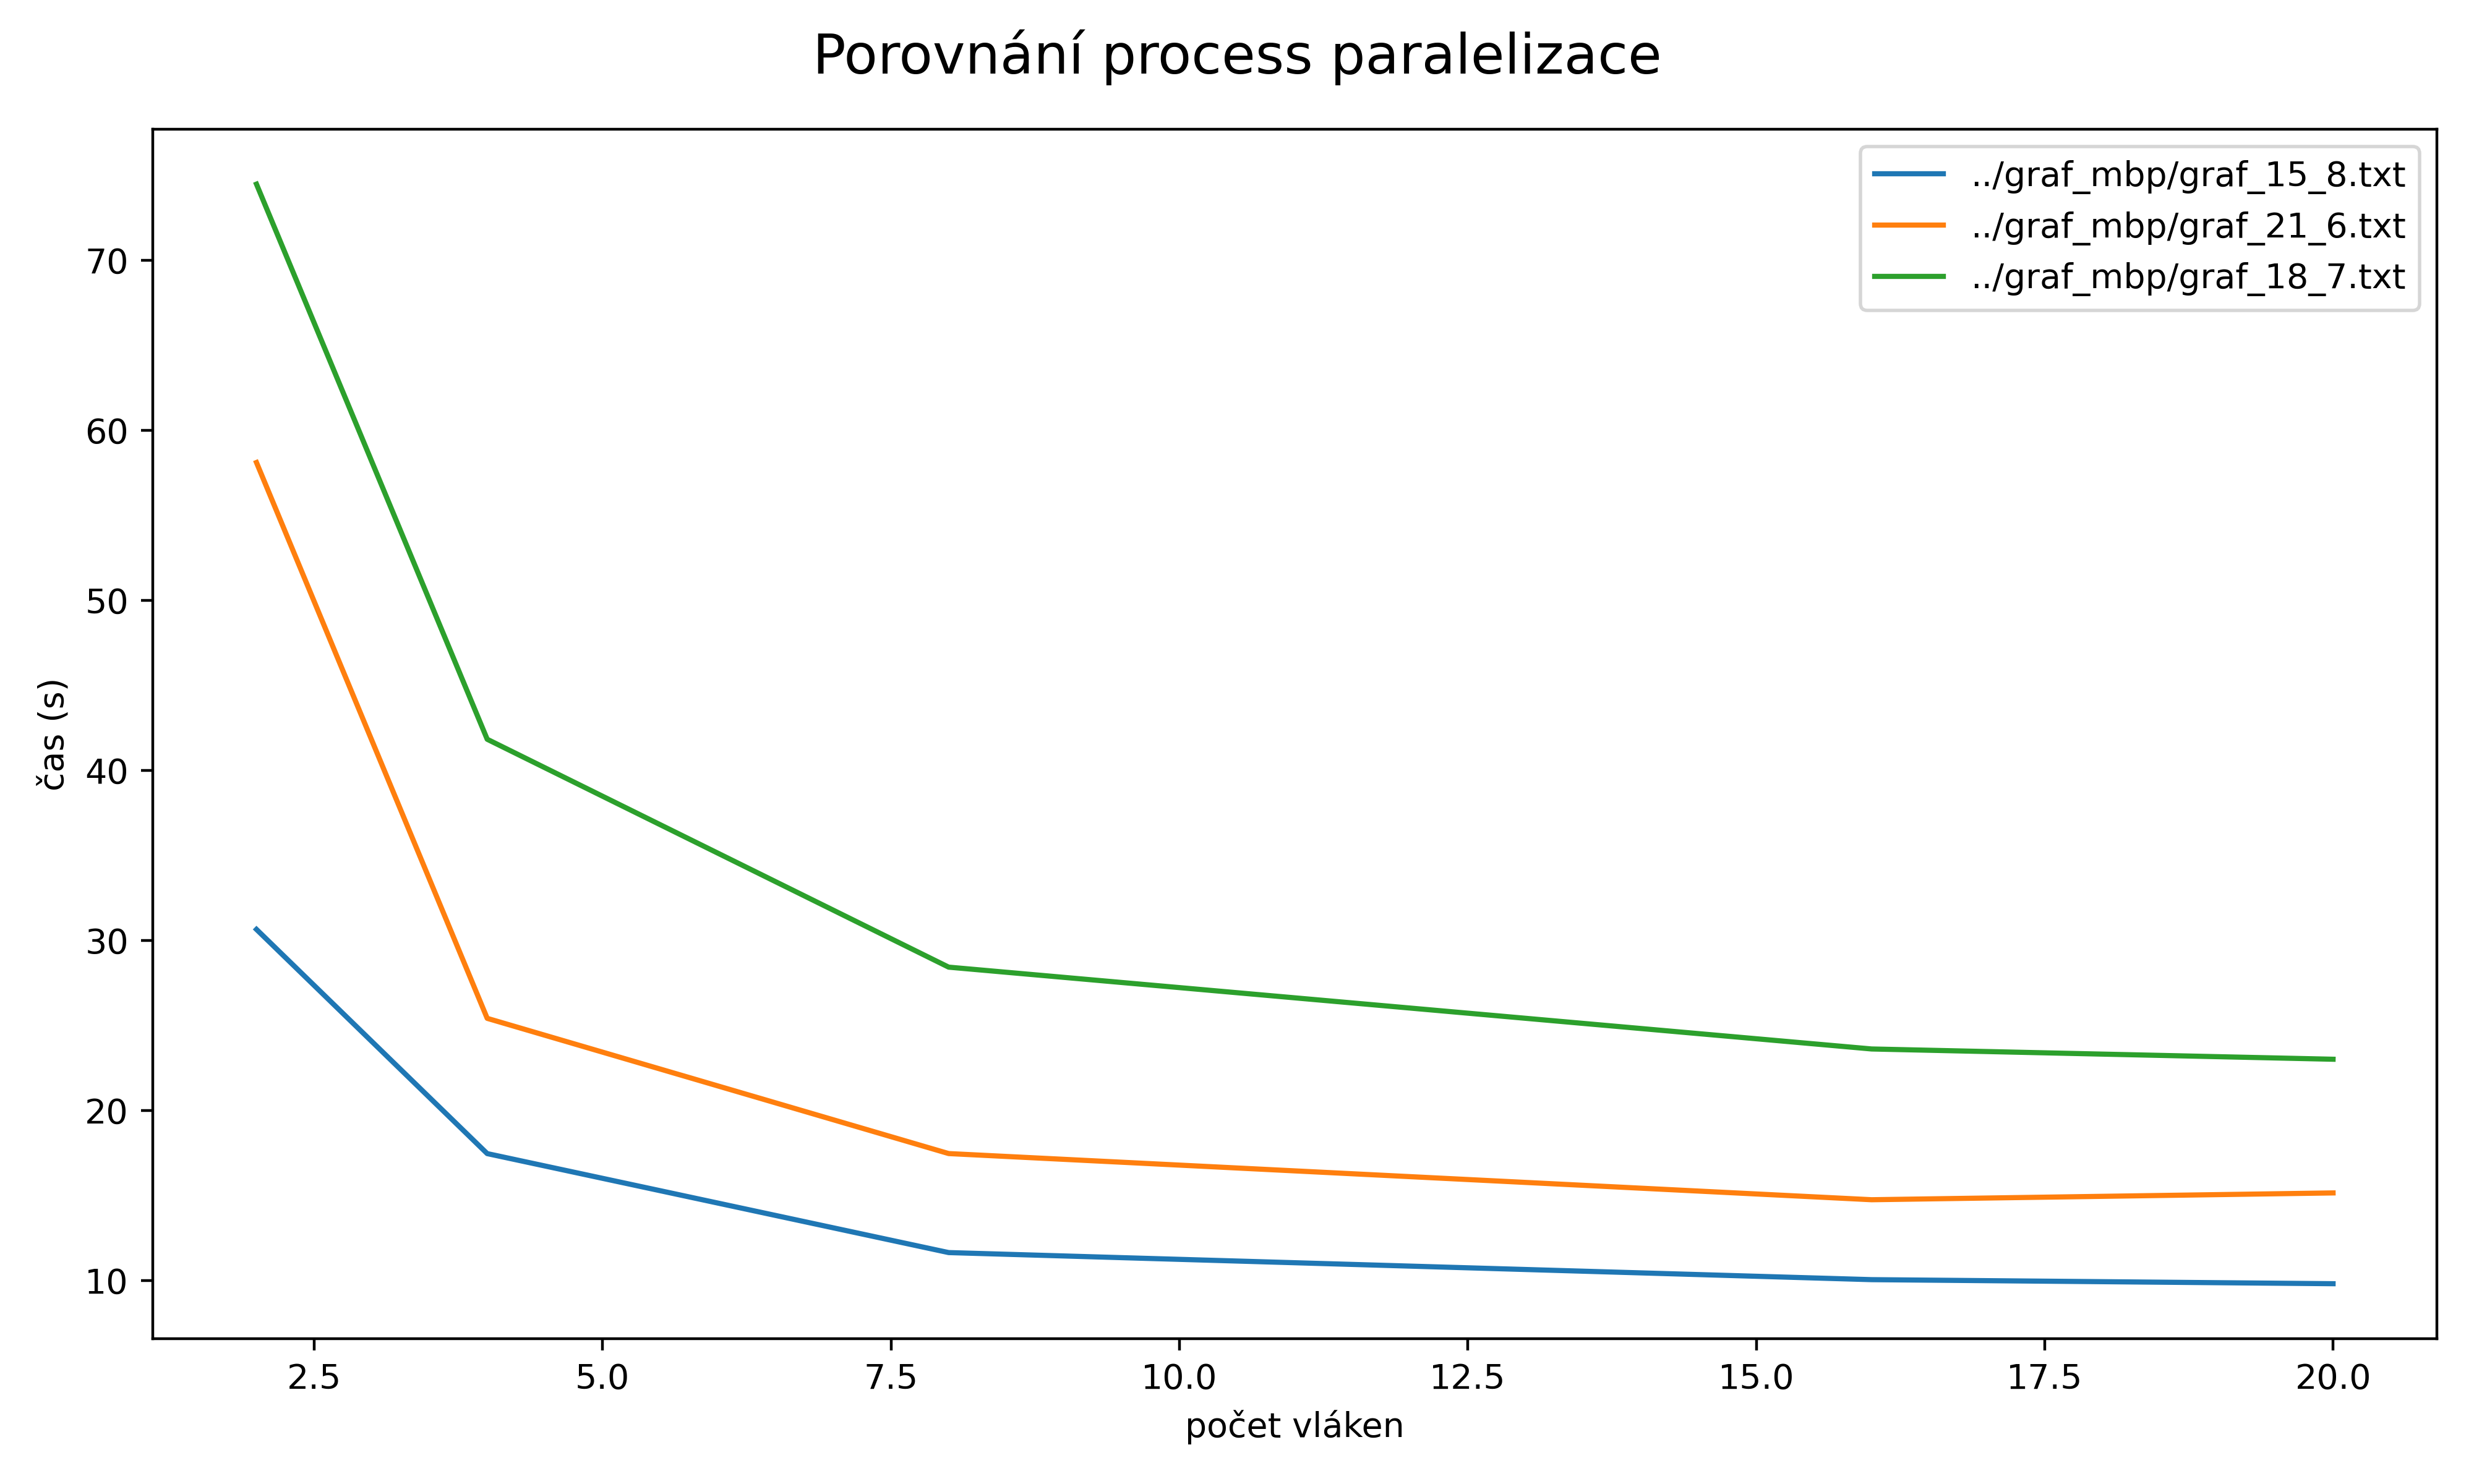
\includegraphics[scale=.46]{images/porovnání_process_paralelizace.png}}
\caption{Škálování MPI paralelizace}
\end{figure}